\section{Architektur}
    \label{section:Architecture}
    Das \gls{wccs} verwendet eine Microservices-Architektur,
    weshalb dieses Muster im folgenden Kapitel vorgestellt wird.
    Anschließend erfolgt die Erläuterung der konkreten Architektur des \glspl{wccs}.

    \subsection{Microservices-Architekturen}
        \label{section:conceptMicroServices}
        Mit "`Microservices"' wird ein Architekturmuster beschrieben,
        dessen grundlegende Idee ist, anstatt eines monolithischen Systems
        ein verteiltes System zu nutzen, bei dem mehrere Prozesse gemeinsam
        eine größere Aufgabe bearbeiten.
        Jeder Prozess wird dabei als "`Service"' bezeichnet und ist darauf
        fokussiert genau eine Aufgabe zu erfüllen.
        Diese Aufgaben sollten möglichst klein sein,
        sodass jeder Service ebenfalls klein gehalten werden kann und seine
        Aufgabe dadurch besonders gut erfüllen kann.
        Die Kommunikation zwischen den Services erfolgt über das Netzwerk
        und definierte Schnittstellen
        \cite[Kapitel 1.1]{newman:microservices}.

        \paragraph{Vorteile}
        Dieses Vorgehen bietet mehrere Vorteile.
        Jeder Service kann verschiedene Technologien einsetzen,
        was zum Beispiel die verwendete Programmiersprache und eingesetzte Frameworks betrifft.
        Services können also unabhängig von einander die Werkzeuge verwenden,
        die am besten zur Erfüllung ihrer Aufgabe geeignet sind
        \cite[Kapitel 1.2.1]{newman:microservices}.
        Die Belastbarkeit des Gesamtsystems steigt,
        da der Ausfall eines Services nicht den Ausfall des restlichen Systems
        zur Folge haben muss
        \cite[Kapitel 1.2.2]{newman:microservices}.
        Werden Services zustandslos gehalten,
        können sie außerdem einfach und unabhängig von einander skaliert werden.
        Im Gegensatz zu Monolithen muss also nicht das ganze System skaliert werden,
        sondern nur die Komponenten, die es erfordern.
        \cite[Kapitel 1.2.3]{newman:microservices}.
        Ein weiterer Vorteil einzelner Services ist,
        dass neue Versionen leichter und mit weniger Risiko als monolithische Systeme
        eingespielt werden können
        \cite[Kapitel 1.2.4]{newman:microservices}.
        Die Entwicklungsarbeit kann zudem leichter aufgeteilt und organisiert werden,
        da für jeden Service ein kleines Team die Verantwortung übernehmen kann.
        Dessen Arbeit ist einfacher, da es für Änderungen nur ihren Service detailliert kennen muss
        und nicht das gesamte System
        \cite[Kapitel 1.2.5]{newman:microservices}.
        Der modulare Aufbau eines solchen Systems erlaubt außerdem, Services
        in Zukunft unterschiedlich wiederzuverwenden
        \cite[Kapitel 1.2.6]{newman:microservices}.
        Bei der Einhaltung einer stabilen Schnittstelle gilt das auch bei einer
        kompletten Neuimplementierung, die durch die geringe Größe von
        Services praktikabel ist
        \cite[Kapitel 1.2.7]{newman:microservices}.       

        \paragraph{Herausforderungen}
        \citet[Kapitel 6.1-6.3]{wolff:microservices} beschreibt aber auch
        Herausforderungen, die die Umsetzung einer Microservices-Architektur mit sich bringen.
        Dies sind vor allem die Latenz und die Unzuverlässigkeit bei der Kommunikation,
        die durch das Netzwerk entstehen.
        Die Entwicklung von Microservices stellt außerdem höhere Anforderungen an die
        verwendete Infrastruktur und den Grad der Automatisierung.

    \subsection{Architektur des WCCS'}
        \label{section:solutionConceptWCCSArch}
        Die Architektur des \glspl{wccs} wird in zwei Schritten vorgestellt.
        Zunächst liegt der Fokus auf dem internen Aufbau des Systems,
        anschließend auf den Zusammenhängen und Interaktionen mit außenstehenden Systemen.
        Da diese Sichten nicht vollständig von einander zu trennen sind,
        tauchen einige Komponenten in beiden Varianten auf.
        
        \paragraph{Interner Aufbau}
        Das \gls{wccs} besteht aus mehreren Komponenten,
        von denen einige Services im Sinne einer Microservices-Architektur darstellen.
        Eine Übersicht der Komponenten ist in Abbildung \ref{image:wccsInternalArchitecture} zu sehen.

        \begin{figure}
            \centering
            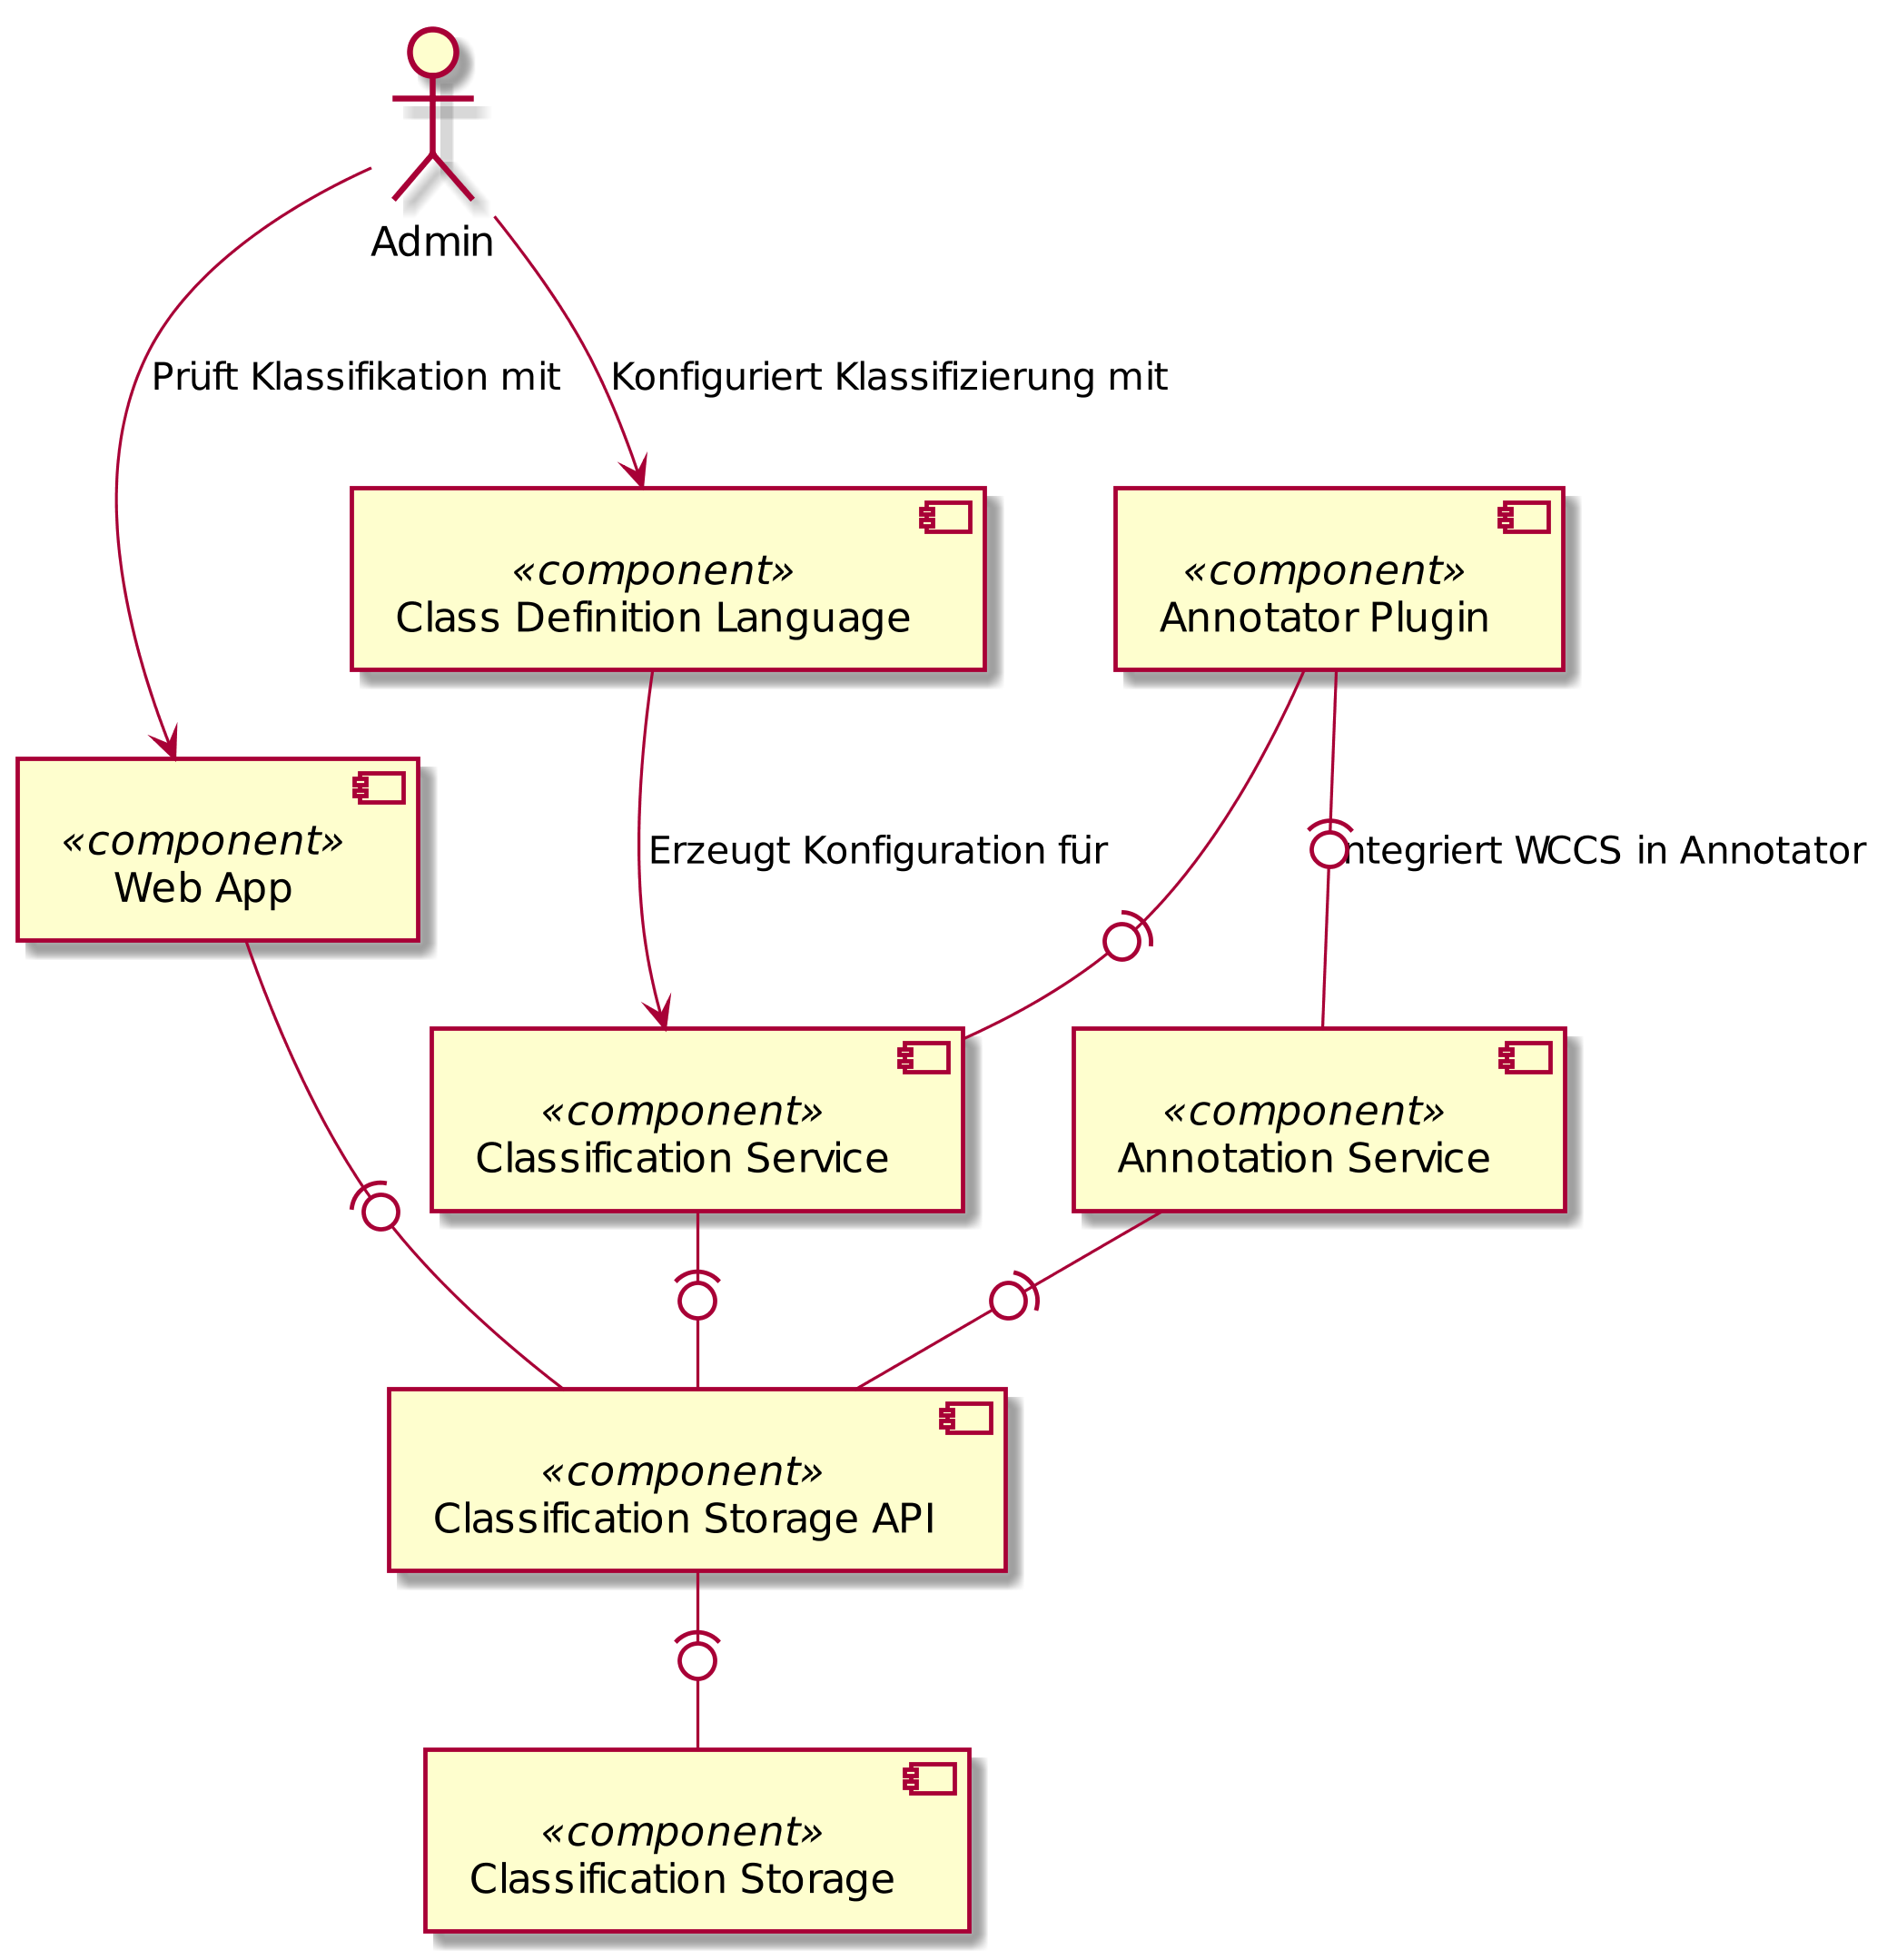
\includegraphics[scale=\imageScalingFactor]{../resources/architecture/wccs_internal_architecture.png}
            \caption{Interner Aufbau des WCCS'}
            \label{image:wccsInternalArchitecture}
        \end{figure}

        Die fünf Services des Systems sind

        \begin{enumerate}
            \item der {\classificationStorage},
            \item die {\classificationStorageAPI},
            \item der {\classificationService},
            \item der {\annotationService} und
            \item die {\webAppService}.
        \end{enumerate}

        Diese Services kommunizieren über HTTP
        und stellen eine Menge von (RESTful) Webservices dar.

        Der {\classificationStorage} stellt die Persistenz bereit und speichert
        Klassifikationen in einer Datenbank.
        Seine Schnittstelle entspricht der der verwendeten Datenbank und ist deshalb
        technisch orientiert.
        Eine ausführliche Darstellung dieser Komponente erfolgt in
        Kapitel \ref{section:solutionDetailsPersistence}.

        Die {\classificationStorageAPI} bietet eine fachliche Schnittstelle zur Datenbank,
        d. h. sie übersetzt fachliche Anfragen in technische Datenbankabfragen und führt diese aus.
        Dementsprechend ist die konkrete Implementierung dieses Services abhängig vom {\classificationStorage}
        und der verwendeten Datenbank.
        Die Schnittstelle der {\classificationStorageAPI}
        ist hingegen unabhängig von der konkreten Datenhaltung,
        da sie sich an der fachlichen Domäne orientiert.
        Drittsysteme nutzen deshalb vorrangig diese Komponente, um die Klassifikation einer Webseite zu beziehen.
        Details der {\classificationStorageAPI} beschreibt Kapitel \ref{section:solutionDetailsStorageAPI}.

        Der {\classificationService} führt die eigentliche Klassifizierung durch
        und speichert das Ergebnis über die {\classificationStorageAPI} dauerhaft.
        Seine Schnittstelle ist ebenfalls fachlich orientiert.
        Kapitel \ref{section:solutionDetailsClassificationService} geht ausführlicher auf diese Komponente
        des Systems und ihre Arbeitsweise ein.

        Der {\annotationService} transformiert eine Klassifikation,
        die er über die {\classificationStorageAPI} bezieht,
        in eine Menge von Annotationen.
        Neben der Abfrage von Annotationen bietet seine Schnittstelle auch
        die Möglichkeit solche zu aktualisieren und damit die Klasse eines Features zu modifizieren.
        Mehr über diesen Service, seine Arbeitsweise und die Rolle seiner Schnittstelle
        erläutert Kapitel \ref{section:solutionDetailsAnnotationService}.

        Der verbliebene Service -- die {\webAppService} -- ist im Kern ein Webserver,
        der die Webanwendung bereitstellt,
        mit der ein Nutzer Klassifikationen prüfen kann.
        Diese bezieht die Anwendung über die {\classificationStorageAPI}.

        Neben diesen Services besitzt das System weitere Komponenten:

        \begin{enumerate}
            \item Die \gls{wccdl} und
            \item das {\annotatorPlugin}.
        \end{enumerate}

        Die \gls{wccdl} nutzt ein Entwickler, um ein {\classificationModel} für den
        {\classificationService} zu erstellen.
        Eine ausführliche Beschreibung der Sprache geschieht in Kapitel \ref{section:solutionDetailsDSL}.

        Das {\annotatorPlugin} stellt eine Integration des \glspl{wccs} in Annotator dar.
        Es bezieht die Annotationen einer Webseite über den {\annotationService}
        und Informationen über bekannte Klassen vom {\classificationService}.
        Beides ist notwendig, um die Visualisierung und Korrektur einer Klassifikation über Annotationen
        zu ermöglichen.
        Diese Komponente wir in Kapitel \ref{section:solutionDetailsAnnotatorPlugin} näher betrachtet.

        \paragraph{Beziehungen zur Außenwelt}
        Die bisherige Betrachtung beantwortet zum Beispiel noch nicht die Frage,
        welche Komponente das Annotator Plugin einbindet und welche sonstigen
        Beziehungen zur Außenwelt das \gls{wccs} besitzt.
        Antworten liefert Abbildung \ref{image:wccsExternalArchitecture},
        die dazu zwischen externen Komponenten und solchen des \glspl{wccs}
        unterscheidet und ihre Beziehungen darstellt.

        \begin{figure}
            \centering
            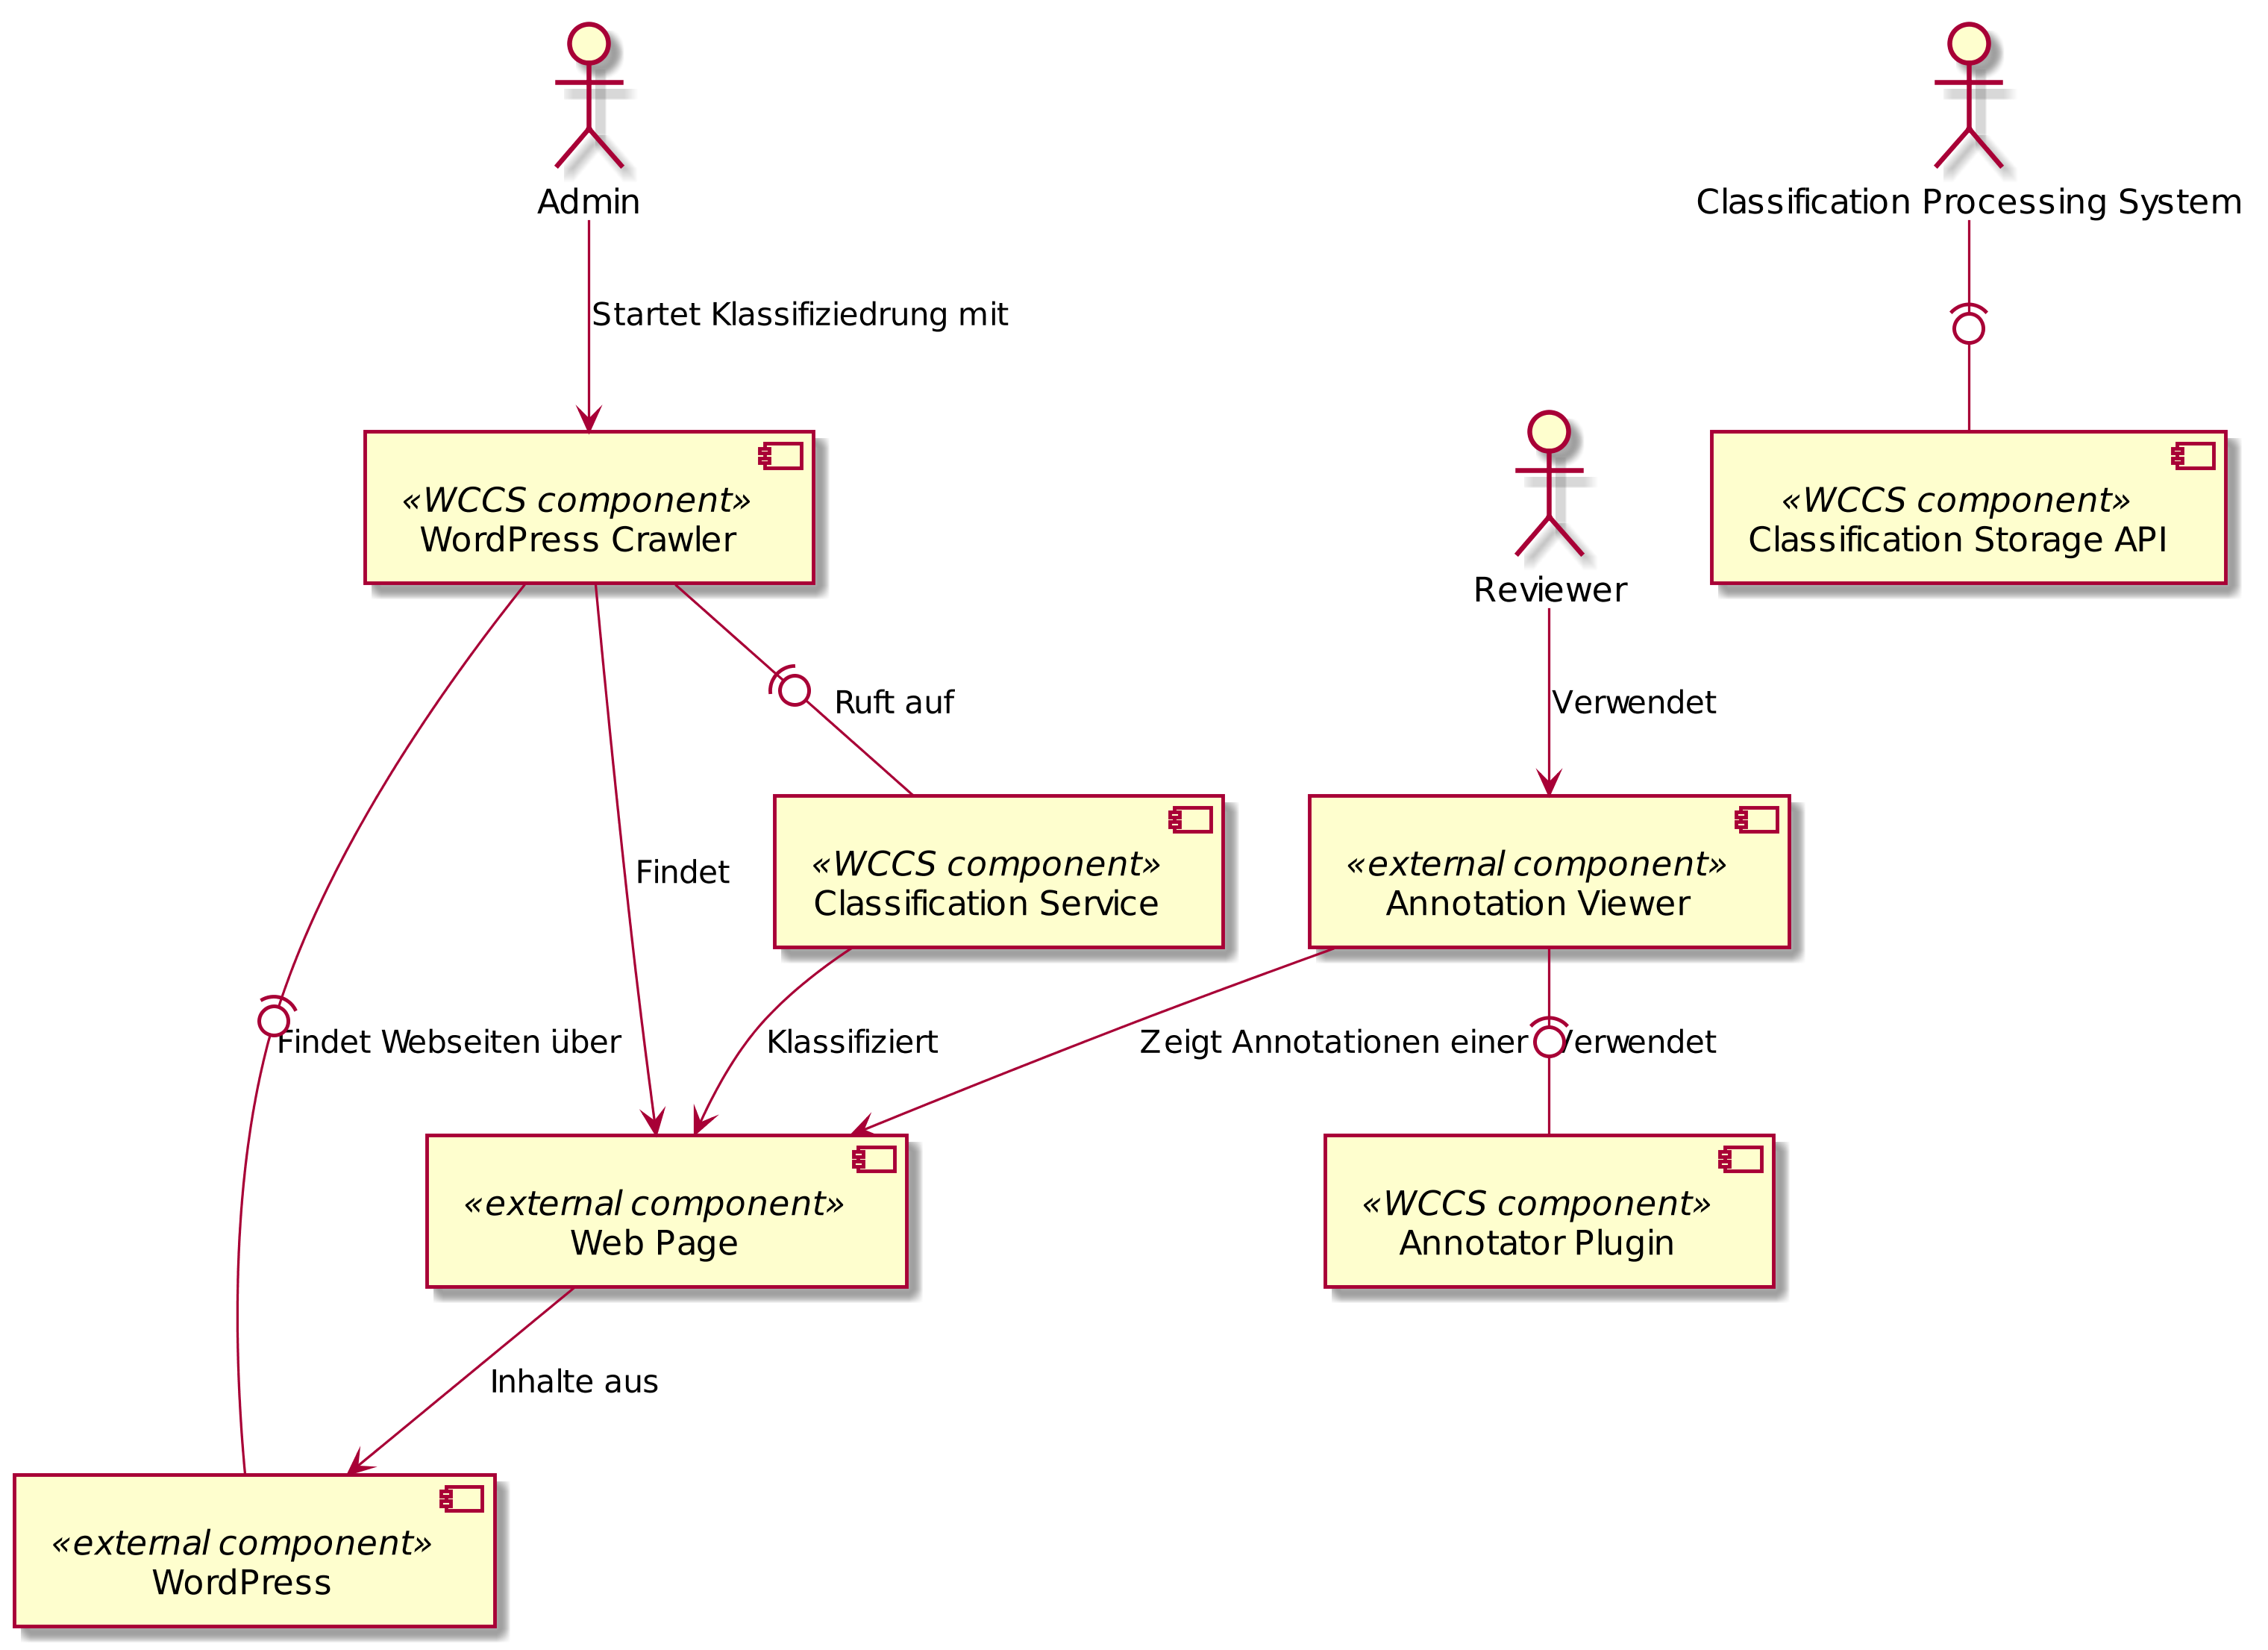
\includegraphics[scale=\imageScalingFactor]{../resources/architecture/external_architecture.png}
            \caption{Beziehungen des WCCS' zur Außenwelt}
            \label{image:wccsExternalArchitecture}
        \end{figure}

        Eine zentrale externe Komponente ist die Webseite,
        die Inhalte aus einem \gls{cms} -- im konkreten Fall {\wordpress} --
        darstellt und vom {\classificationService} klassifiziert wird.
        
        Dazu startet ein Anwender den {\wordpressCrawler}, der ebenfalls ein Teil des \glspl{wccs} ist.
        Diese Komponente findet Webseiten über {\wordpress}' RESTful Webservice und beauftragt den
        {\classificationService} diese zu klassifizieren.
        Obwohl der {\wordpressCrawler} zum \gls{wccs} gezählt wird,
        stellt er nur eine Beispielimplementierung dar,
        da er aufgrund seiner engen Kopplung zu {\wordpress} weniger allgemeingültig ist.
        Unabhängig davon ist die konzeptionelle Notwendigkeit einer Komponente,
        die zu klassifizierende Webseiten ermittelt.
        Der {\wordpressCrawler} wird in Kapitel \ref{section:solutionDetailsCrawler} nochmals betrachtet.

        Nach ihrer Klassifizierung kann eine Webseite das {\annotatorPlugin} einbinden
        und damit die Klassifikation über Annotationen visualisieren.
        Anwender können dann die Klassifikation prüfen und bei Bedarf modifizieren,
        wozu sie die Funktionen des {\annotatorPlugin}s verwenden.
